\setcounter{page}{2}
\tableofcontents
\newpage

\section*{Введение}
\addcontentsline{toc}{section}{Введение}
В настоящее время происходит постоянное увеличение сфер применения программного обеспечения, увеличивается количество устройств, оснащенных процессорами, что ведет к значительному росту числа программных и аппаратных платформ. Если несколько лет назад программам было достаточно работать под управлением ОС Windows на процессоре семейства Intel x86, то сейчас программистам необходимо уметь подготовить свой проект для работы на 4-5 программно-аппаратных платформах. В качестве основных факторов, расширивших спектр платформ, можно назвать следующие:

\begin{itemize}
\item Активное расширение рынка мобильных устройств со своими операционными системами, библиотеками и архитектурами процессоров
\item Конкуренция на рынке настольных операционных систем, вследствие которой все большее количество пользователей устанавливает на свои компьютеры не Microsoft Windows, а альтернативные ОС, например, Linux
\item Активное развитие систем, где традиционный набор <<Windows-Intel x86>> не является оптимальным - например, в системах с автономным питанием или в высокопроизводительных системах
\end{itemize}

Исходя из этих факторов, можно сделать вывод, что наибольшего успеха могут добиваться разработчики, предлагающие свои программные продукты для нескольких программных и аппаратных платформ, и способные в короткие сроки добавлять поддержку новых ОС и процессоров в свои проекты. В связи с этим возникает проблема обеспечения поддержки продуктом сразу нескольких программных платформ.
Проблема поддержки нескольких программных и аппаратных платформ может быть решена следующими способами:
\begin{itemize}
	\item Созданием платформо-независимого программного слоя, способного обеспечить сборку программы для различных платформ из единой кодовой базы;
	\item Использованием платформо-независимых библиотек абстракций, таких как Qt
	\item Осуществлением портирования (миграции, переноса) продукта на новую платформу
\end{itemize}

Первый подход достаточно трудоемок и требует от разработчиков предварительного исследования особенностей возможных целевых платформ. Разработка и поддержка платформо-независимого программного слоя требует дополнительных трудозатрат и могут увеличить сроки и бюджет разработки. Этот подход может успешно применяться в крупных компаниях, имеющих отдел исследований и несколько отделов разработки, которые позволяют им сократить время разработки программного слоя и окупить разработку слоя за счет его использования в линейке собственных программных продуктов.

Второй подход наиболее прост для разработчиков, но имеет недостатки. Во-первых, программы должны изначально разрабатываться с учетом использования платформо-независимых библиотек абстракций. Переписывание уже существующей программы на базе одной из платформо-независимых библиотек по трудоемкости сравнимо с первым подходом. Кроме того, платформо-независимые библиотеки предоставляют ограниченный набор абстракций, а добавление новых возможностей в одну из существующих библиотек зачастую вызывает больше сложностей, чем создание собственного программного слоя.

Третий подход предполагает адаптацию программы или её компонента с целью обеспечения их работы в среде, отличающейся от среды, для которой изначально создавалась программа, при сохранении соответствия функциональным и нефункциональным требованиям к оригинальной программы. Портирование позволяет расширять список целевых платформ по мере необходимости и позволяет на ранних этапах разработки не задумываться о поддержке всего многообразия платформ. Процесс портирования требует от программиста высокой квалификации и понимания принципов работы оригинальной программы, а также дополнительных временных затрат на проверку качества полученной программы.

При обновлении версий используемых программой библиотек, из-за потери обратной совместимости, могут возникать задачи, сходные с задачей портирования, и они также могут быть решены с помощью технологий, применяемых при портировании.

В ходе данной работы будут проанализированы подходы к задаче миграции программ на новый набор библиотек, существующие инструменты для этого и проблемы, стоящие при создании собственного инструмента миграции.

\section{Обзор методов миграции программ}
Рассмотрим следующую ситуацию. Имеется программная система, разработанная для определенного набора библиотек. Необходимо портировать программу на другой набор библиотек (в частности, адаптировать программу для новой ОС), не переписывая программу с нуля. Проанализируем подходы к этой задаче, и для каждого подхода рассмотрим хотя бы один пример его реализации.

Существующие подходы к проблеме миграции программ можно разделить на следующие группы:
\begin{itemize}
	\item Трансляция вызовов (эмуляция ABI)
	\item Виртуализация уровня ОС
	\item Создание обёрток (wrappers, эмуляция API)
	\item Синтаксический подход
	\item Семантический подход
\end{itemize}

Первые три группы можно отнести к динамическим подходам, а оставшиеся две~-- к статическим.

Для сравнения различных подходов были выбраны следующие критерии оценки:

\begin{itemize}
	\item Тип подхода - статический или динамический. В случае динамических подходов миграция происходит во время выполнения программы (т.е. миграция выполняется заново при каждом запуске), что, как правило, оказывает негативное влияние на производительность. Статические подходы производят миграцию один раз.
	\item Объект миграции - исполняемый или исходный код.
	\item Влияние на производительность портированной программы
	\item Сложность адаптации для новых библиотек - насколько система миграции, созданная в соответствии с исследуемым подходом, привязана к конкретной библиотеке
	\item Доступ к объектам целевой библиотеки - возможность использования API новой библиотеки из портированного кода
\end{itemize}

\subsection{Трансляция вызовов}
Существует несколько программных решений, позволяющих запускать исполняемые файлы, созданные для других операционных систем, путем использования транслятора, способного считывать и разбирать файлы требуемого формата, преобразуя вызовы функций, осуществляемые внутри файла, в соответствующие вызовы текущей ОС. Фактически, такой транслятор реализует бинарный интерфейс (ABI) старой системы в новой системе.

В качестве примера реализации данного подхода можно привести утилиту Wine, предназначенную для запуска Windows-приложений в ОС Linux.

Wine (Wine Is Not Emulator) не является эмулятором операционной системы: он не создаёт изолированной среды для выполнения и не обеспечивает доступ к низкоуровневым системным ресурсам, таким как непосредственный доступ к оборудованию. Функция Wine состоит в том, чтобы, с одной стороны, предоставить Windows-приложению Win API — стандартный системный интерфейс операционных систем Windows, а с другой стороны, транслировать запросы Windows-приложения в соответствующие системные вызовы (POSIX API). Wine работает на различных Unix-системах, в том числе на Linux. Таким образом, Wine — это своеобразная «прослойка» совместимости между Windows-приложениями и Unix хост-системой.

Процесс Wine всегда выполняется в непривилегированном режиме и не требует никакой модификации ядра операционной системы (в том числе динамически загружаемых модулей). Любые проблемы, которые могут быть вызваны запуском win-приложений, будут ограничены правами доступа того пользователя, который запустил Wine. В результате Windows-приложения будут подчиняться политике доступа Unix-системы и не смогут её нарушать.

У данного ограничения есть и другая сторона: в Wine нет поддержки низкоуровневого обращения к оборудованию (драйверам оборудования, прямой работы с USB-устройствами). Всё периферийное оборудование следует подключать и настраивать в хост-системе: для Windows-приложений эти устройства могут быть доступны стандартным способом через файловую систему или другие стандартные интерфейсы (например, TWAIN для сканеров, который реализован в Wine как обёртка над библиотекой SANE).

Wine состоит из нескольких компонент, которые условно можно поделить на три части:

\begin{itemize}
	\item libwine - библиотека, предоставляющая Win API для Windows-приложений. По количеству предоставляемых функций её можно сравнить с Qt — столь широк спектр предлагаемых вызовов: от операций с файлами до построения графического интерфейса и обращения к базам данных.
	\item wine - Среда для исполнения двоичных win-приложений, предоставляет программам окружение, неотличимое от Windows. Это окружение помимо Win API включает реестр, стандартные каталоги и файлы.
	\item Утилиты, имитирующие некоторые стандартные win-приложения: текстовый редактор (блокнот), файловый браузер и т. п. Средства компиляции и отладки: имеются заголовочные файлы, которые описывают доступное API, компилятор winegcc, представляющий собой обёртку над gcc, отладчик winedbg и прочие вспомогательные утилиты.
\end{itemize}

Wine — это свободный проект, который был начат в 1993 году. На тот момент распространённой платформой была Win16 (Windows 3.1), на неё и был ориентирован Wine, на сегодняшний день основное русло разработки — Win32. Исходные тексты Wine выпускаются под лицензией LGPL (Lesser GPL), никаких ограничений по доступу к исходным текстам и их модификации не имеется.

Удобство данного подхода (и его реализации в виде Wine) заключается в том, что при этом не требуется перекомпилировать приложение — один и тот же исполняемый файл годится и для Windows, и для Wine.

\subsection{Виртуализация уровня ОС}
Эмуляция (emulation) — имитация функционирования одного устройства посредством другого устройства или устройств вычислительной машины, при которой имитирующее устройство воспринимает те же данные, выполняет ту же программу и достигает того же результата, что и имитируемое.

Альтернативой трансляции вызовов некоторой системы является запуск копии такой системы внутри основной ОС, с использованием программ, эмулирующих аппаратное обеспечение — виртуальных машин. На такой машине устанавливается операционная система и другое окружение, необходимое приложению, а само приложение запускается уже в родной для него среде.

Возможность запуска приложения на виртуальной машине зависит, в основном, от возможностей самой машины, нежели от разработчиков приложения. Тем не менее, программы, работающие с аппаратурой напрямую, могут встретить определенные трудности, поскольку им будет предоставлен доступ к устройствам виртуальной машины, а не непосредственно компьютера. Такая особенность ограничивает, например, возможность работы с графическими ускорителями изнутри виртуальных машин.

В общем случае использование виртуальной машины достаточно ресурсоемко — ведь помимо собственно приложения, ресурсы компьютера потребляются самой машиной, а также работающими внутри нее программами, необходимыми для функционирования приложения (например, операционной системой). Поэтому выигрыш в производительности достигается, как правило, только в случае запуска машин, эмулирующих достаточно маломощные платформы на более производительных системах.

Проблеме производительности виртуальных машин уделялось много внимания еще в 70-е годы. Впервые требования, которым должна удовлетворять аппаратная архитектура машины, чтобы на ней можно было эффективно реализовать виртуализацию, были сформулированы Попеком и Голдбергом в 1974 году \cite{popek1974formal}. Основное требование сводится к разделению всех инструкций по разным уровням привилегий; при этом все инструкции, способные изменить состояние ресурсов виртуальной машины, а также инструкции, поведение которых зависит от конфигурации этих ресурсов, должны быть привилегированными. Монитор виртуальных машин (Virtual Machine Monitor, VMM — программная прослойка, занимающаяся распределением физических ресурсов между работающими виртуальными машинами), сам работая с наивысшими привилегиями, может перехватывать эти инструкции и эмулировать их поведение в соответствии со своими потребностями. Все непривилегированные инструкции должны выполняться непосредственно на аппаратуре. Поскольку доля привилегированных инструкций, как правило, невелика, то и затраты на их эмуляцию будут малы.

Несмотря на то, что статья Голдберга и Попека написана более 40 лет назад, во времена таких машин, как IBM 360 или DEC PDP-10, сформулированные в ней требования справедливы и сегодня. Например, для архитектуры x86 к числу таких инструкций относятся такие инструкции, как push/pop, call, jmp и некоторые другие (более подробно данная проблема рассмотрена в \cite{kasp}).

Рассмотренный принцип разделения инструкций реализован в таких системах, как VirtualBox\cite{virtualbox} и VMWare\cite{vmware}. В целях повышения быстродействия, эти системы напрямую выполняют все непривилегированные инструкции. Тем не менее, необходимость дополнительного отслеживания выполняемых инструкций может замедлить производительность программ внутри виртуальной машины по сравнению с хост-системой.

Осознание разработчиками важности виртуализации привело к появлению расширений от Intel (Intel Virtualization Technology\cite{vtx}) и AMD (AMD Virtualization\cite{amd}) для ее поддержки на платформах x86 и x86-64, которые позволяют либо вовсе избавится, либо существенно снизить число перехватываемых и эмулируемых инструкций.

Важным моментом при использования виртуальной машины является экономическая составляющая — в ряде случаев стоимость лицензий на операционную систему и компоненты окружения, которые необходимо установить, может быть довольна значительна.

\subsection{Обертки}

Обертка (wrapper) - это программный модуль, который соответствует программному интерфейсу (API) одной библиотеки, но реально не содержит никакой логики, вместо этого он передает управление другой библиотеке. Фактически обертки являются трансляторами вызовов, работающими на уровне исходного кода. В объектно-ориентированных языках обертки называются паттерном проектирования <<Адаптер>>.

\begin{figure}[H]
	\centering
	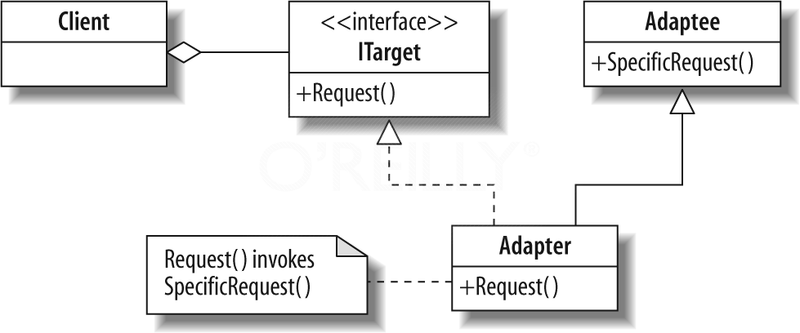
\includegraphics[width=0.8\textwidth]{adapter.png}
	\caption{UML-диаграмма классов для паттерна <<Адаптер>>}%
\end{figure}

Ниже приведен пример обертки на языке C++. Допустим, новая библиотека сообщает о текущей температуре в градусах Фаренгейта, а код в проекте рассчитан на то, чтобы получать температуру в градусах. В таком случае необходимо добавить в программный проект следующий код:

\begin{lstlisting}[language=C++]
class FahrenheitSensor
{
  public:
    float getFahrenheitTemp() {
      float t;
      // ...
      return t;
    }
};
  
class Sensor
{    
  public:
    virtual ~Sensor() {}
    virtual float getTemperature() = 0;
};
  
class Adapter : public Sensor
{    
  public:
    Adapter( FahrenheitSensor* p ) : p_fsensor(p) {
    }
   ~Adapter() {
      delete p_fsensor;
    }
    float getTemperature() {
      return (p_fsensor->getFahrenheitTemp()-32.0)*5.0/9.0;
    }
  private:
    FahrenheitSensor* p_fsensor; 
};
  
int main()
{
  Sensor* p = new Adapter( new FahrenheitSensor);
  cout << "Celsius temperature = " << p->getTemperature() << endl;
  delete p;    
  return 0;
}
\end{lstlisting}

Основной недостаток оберток - тот факт, что они проектируются для конкретных библиотек. Если исходная или целевая библиотека изменятся, обертку придется переписывать с нуля. Кроме того, обертки несколько уменьшают производительность работы кода и ограничивают доступ к объектам целевой библиотеки.

\subsection{Синтаксический подход}
Синтаксические подходы в процессе миграции кода используют информацию о синтаксисе языка программирования. К этой группе относятся подходы на основе шаблонных преобразований и перезаписи термов.

В подходах, основанных на шаблонных преобразованиях, по исходному коду строится модель и определяются шаблоны заменяемого кода. В процессе трансформации осуществляется поиск кода по шаблону и применение к нему трансформаций. Основными различиями в таких подходах являются используемые модели кода, языки описания шаблонов и способы задания трансформаций. Примером средства на основе шаблонных преобразований может служить интегрированная среда разработки IntelliJ IDEA.

Система шаблонных преобразований в IntelliJ IDEA изначально разработана для поиска и исправления ошибок в коде, но может использоваться и для миграции программ. Довольно большое количество шаблонов изначально содержится в IDEA, однако имеется возможность добавить свои шаблоны с помощью функции Structural Search and Replace\cite{ideaSSR}. Данная функция во многом похожа на обычный диалог замены текста (Search and Replace), однако учитывает синтаксис кода. Например, при поиске вхождения не учитывается разница в форматировании между шаблоном поиска и исходным кодом, а также не учитывается порядок объявления переменных, методов, полей и некоторых других синтаксических конструкций.

Если нет необходимости искать точное совпадение, в шаблоне можно использовать переменные, в таком случае на месте шаблона в искомом коде может находиться произвольный текст. Переменные обозначаются с помощью двух знаков \$, как на рисунке \ref{fig:ssr}.

\begin{figure}[H]
	\centering
	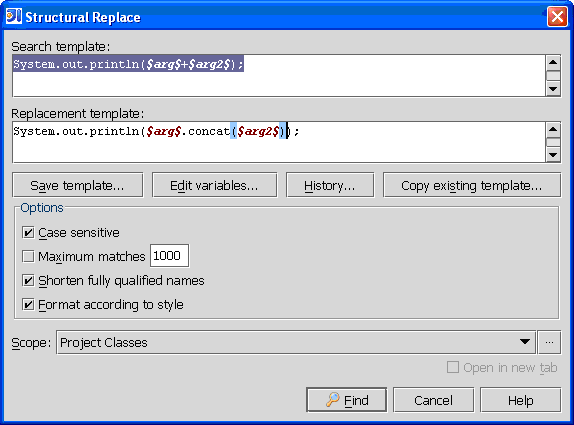
\includegraphics[width=0.8\textwidth]{ssr.png}
	\caption{Пример использования переменных в шаблонах поиска}%
	\label{fig:ssr}
\end{figure}

При этом есть возможность указывать ограничения для каждой переменной: регулярное выражение, которому она должна соответствовать, минимальное и максимальное число элементов программы, которые могут входить в переменную, и так далее.

Большинство синтаксических методов основывается на использовании правил перезаписи. Абстрактная система перезаписи включает множество объектов, над которыми выполняется перезапись, и множество отношений, которые задают возможные преобразования элементов множества объектов друг в друга. Одним из представителей этой группы является язык TXL\cite{cordy2006txl}. В его основе лежит система перезаписи термов, взаимодействие с которой осуществляется с помощью специального функционального языка программирования. Для задания отношений и правила перезаписи задаются на этом языке, а для задания множества объектов в TXL используется расширенная форма Бэкуса — Наура.

Развитием подхода правил перезаписи является концепция стратегий перезаписи. Данная концепция легла в основу языка трансформации Stratego, реализованного в рамках системы Stratego/XT\cite{bravenboer2008stratego}. В данной системе в качестве модели программы, над которой выполняется трансформации, используются аннотированные термы. Таким образом, при построении абстрактного синтаксического дерева программы система получает дополнительно информацию о семантике терма, которая затем может быть использована в правилах перезаписи.

В статье \cite{broeksema2011visual} рассмотрено использование синтаксического подхода непосредственно для портирования программ. Авторы статьи составили набор правил перезаписи и в рамках тестирования частично портировали проект kdelibs с библиотеки Qt версии 3 на Qt 4.

Основной недостаток синтаксических подходов - их малая гибкость. С помощью этих подходов можно выполнить только простейшие преобразования - замена вызова одной функций на другую, перестановка двух аргументов функции местами и другие преобразования, затрагивающих лишь один или несколько операторов. Более масштабные изменения в случае синтаксических подходов либо требуют написания крайне сложных шаблонов, либо вовсе невозможны.

\subsection{Семантические подходы}
\begin{figure}[htbp]
	\centering
	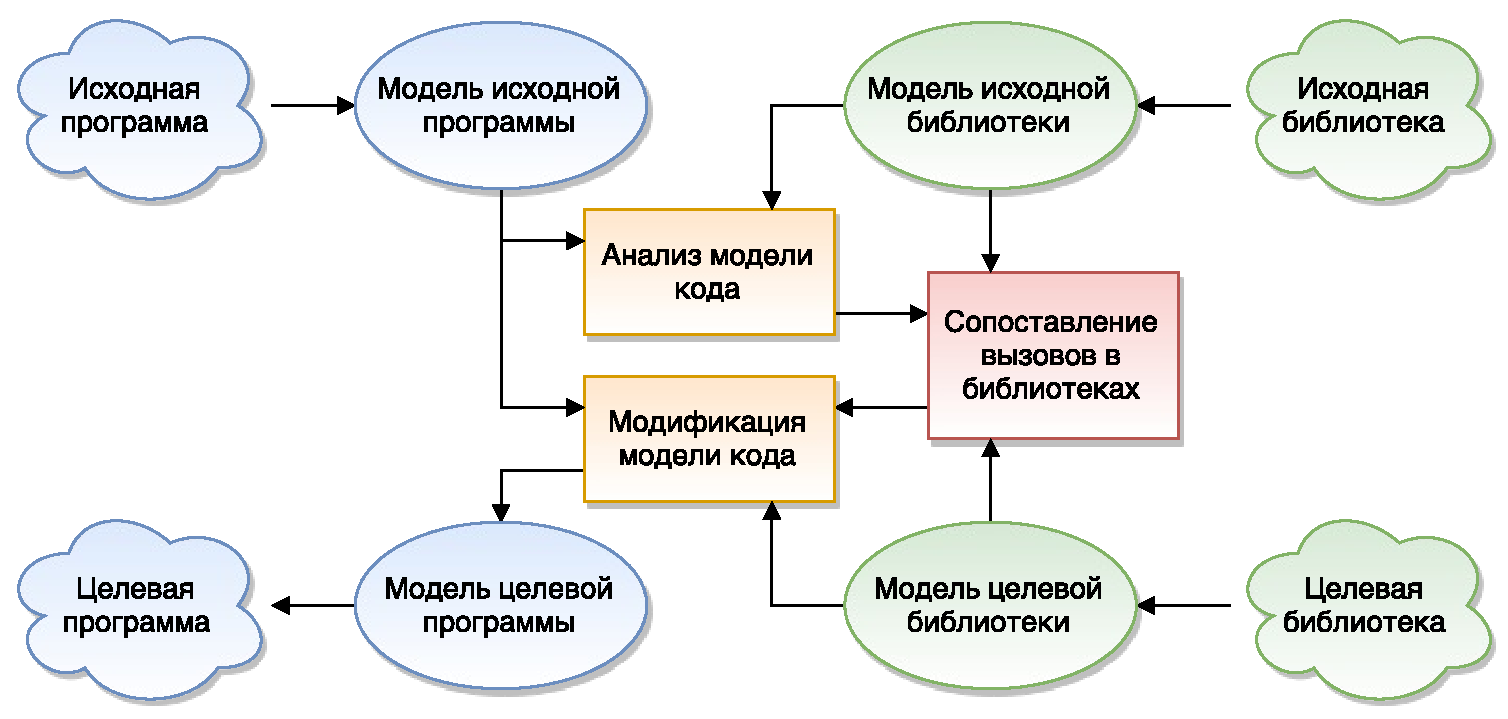
\includegraphics[width=\textwidth]{scheme.pdf}
	\caption{Общая схема работы семантических подходов}
\end{figure}

Семантические подходы являются развитием синтаксических подходов. Наличие описанной семантики библиотеки позволяет выполнять значительно более сложные преобразования, затрагивающие целые функции.

В данных подходах вместо шаблонов преобразования используются семантические описания библиотек (модели библиотек). На основе данных описаний рассчитываются изменения, которые необходимо внести в код. Информация, содержащаяся в модели библиотеки, зависит от конкретной системы миграции.

Модель библиотеки по своей сути является спецификацией библиотеки. Существует два вида спецификаций для библиотек - полные и частичные. Для того, чтобы составить полную спецификацию какой-либо библиотеки, требуется описать её внешние воздействия на окружение и все внутренние аспекты реализации. Такая спецификация в большинстве случаев будет более громоздкой, чем непосредственно исходный код библиотеки. Применение полных спецификаций при автоматизации портирования нецелесообразно, так как их правильное составление займет больше времени, чем портирование программы вручную. Кроме того, при портировании программ на новый набор библиотек, такое подробное описание не требуется и может только помешать анализу. Для портирования программ достаточно описать лишь часть свойств, характеризующих взаимодействие библиотеки с программой и внешним окружением (другими словами, использовать частичные спецификации).

Библиотеки и окружение могут взаимодействовать с программой следующими  способами:
\begin{itemize}
	\item Через аргументы функций;
	\item Через возвращаемое значение функции;
	\item Через глобальные переменные программы.
\end{itemize}

В частичных спецификациях должна быть возможность учесть эти типы влияния и описать семантику любого действия с глобальным и локальными переменными. Подобное описание позволит производить анализ на основе семантики и автоматизировать портирование программ.

Для задания семантики окружения в частичных поведенческих спецификациях могут быть применены следующие механизмы:

\begin{itemize}
	\item семантическая интерпретация типов. Суть механизма заключается в связывании типа языка с семантиками его использования. Механизм может использоваться для задания совместимых типов языка;

	\item семантическая интерпретация значений переменных. Суть механизма заключается в связывании значения переменной с некоторой семантикой. Механизм может использоваться для задания диапазонов допустимых значений переменных и значений, свидетельствующих об ошибке;

	\item параметризуемые абстрактные действия функций. Суть механизма состоит в описании семантики функций в виде набора действий. Такое описание позволяет сопоставить семантики библиотечных подпрограмм, а также контролировать глубину раскрытия семантики.
\end{itemize}


Пример системы, разработанной в соответствии с данным подходом - <<Технология автоматизации трансформации программ при миграции в новое библиотечное окружение>> \cite{baun}. Для описания моделей библиотек в этой системе использовался язык PanLang \cite{panlang}, разработанный на кафедре КСПТ. В ходе работы было показано, что семантические подходы могут быть реализованы в программном инструменте и корректно работают для выбранных портируемых программ. Однако язык PanLang и вытекающая из него модель библиотек подходят только для процедурных языков и не всегда позволяют в достаточной степени описать семантику библиотеки, что сильно ограничивает применимость технологии.

Другой пример подобной системы описан в статье \cite{christoph2003great}. Для описания библиотек использовался язык UML. Авторы статьи сосредоточились на миграции структур данных, оставив за рамками своей работы миграцию логики работы. Кроме того, семантическое описание во многом ориентируется на единственную библиотеку - EJB, что ещё сильнее ограничивает спектр применения разработанной системы.

Семантические подходы не уменьшают производительность портированного кода по сравнению с оригинальным и не ограничивают его доступ к объектам новой библиотеки. Однако, как видно из приведенных примером систем, очень многое в данном подходе зависит от используемой модели библиотеки. Если модель не позволяет в достаточной степени описать библиотеку, применимость данного подхода резко снижается.

Итоговое сравнение: \\

\begin{tabular}{|p{3cm}|p{1.2cm}|p{2cm}|p{3cm}|p{3cm}|p{3cm}|}
	\hline
	Название подхода & Тип & Объект миграции & Влияние на производительность & Сложность адаптации для новых библиотек & Доступ к объектам целевой библиотеки \\ 
	\hline
	Виртуализа- ция & Дин. & Исполн. код & Высокое & Низкая & Ограничен \\
	\hline
	Трансляция вызовов & Дин. & Исполн. код & Среднее & Высокая & Ограничен \\
	\hline
	Обертки & Дин. & Исходн. код & Среднее & Средняя & Ограничен \\
	\hline
	Синтаксич. подход & Стат. & Исходн. код & Низкое & Высокая & Не ограничен \\
	\hline
	Семантич. подход & Стат. & Исходн. код & Низкое & Средняя & Не ограничен \\
	\hline
\end{tabular} \\

В результате можно сделать вывод, что для указанных критериев оптимальным является использование семантического подхода.

\section{Обзор инструментов трансформации программ}
К сожалению, инструментов, реализующих семантический подход, достаточно мало. Сложно провести полноценный анализ проблем, возникающих при проектировании подобных инструментов, поэтому рассмотрим более общую задачу трансформации программ (program transformation) и инструменты, которые её реализуют. Многие вопросы, возникающие при трансформации программ, актуальны для задачи портирования с помощью семантического подхода.

Инструмент трансформации программ является так называемым транспайлером (transpiler, transcompiler, source-to-source compiler) - компилятором, результатом работы которого является код на высокоуровневом языке (в отличие от обычных компиляторов, которые на выходе дают программу в машинных кодах или на языке ассемблера). Помимо миграции, транспайлеры используются для решения следующих задач:

\begin{itemize}
\item Трансляция программ на другой язык программирования. Например, первый компилятор языка C++ (Cfront, 1983 г.) являлся именно транспайлером. Сначала программа на C++ транслировалась в программу на C, после чего собиралась одним из существующих компиляторов языка C. Как правило, трансляция возможна только для родственных языков (например, транспайлер является основным средством сборки для языков CoffeeScript, Haxe и TypeScript). Существуют проекты трансляторов для неродственных языков, но написание такого транспайлера является достаточно трудоемкой задачей.

Примером транслятора, работающего между неродственными языками, может служить J2ObjC. Это средство предназначено для трансляции кода на языке Java в код на языке Objective-C для платформы iOS. Основным применением средства является совместное использование бизнес-логики и логики доступа к данным, описанной на языке Java, на различных платформах, таких как Android и iOS. Средство позволяет использовать в коде многие возможности Java, такие как потоки, исключения, анонимные классы и рефлексию. Также оно позволяет транслировать использующие библиотеку JUnit модульные тесты.

Еще одним примером может служить средство Emscripten\cite{zakai2011emscripten}. Оно позволяет транслировать байткод LLVM в код на языке JavaScript. С помощью данного средства были портированы многие крупные проектов с открытым исходным кодом. Байткод LLVM может быть получен из языков C, C++, Objective-C и др. с помощью компиляторов GCC и Clang. Байткод может быть получен из скомпилированной версии библиотеки, но при этом в нем нет информации о том, из чего байткод был получен, что позволяет средству генерировать только однофайловые программы.
\item Перенос программ на другую версию языка. Пример инструмента для переноса на более новую версию языка - скрипт 2to3, транслирующий программу на языке Python 2 в программу на языке Python 3. Третья версия языка Python не имеет обратной совместимости со второй версии, и поэтому разработчикам необходимо переписывать старые программы, чтобы иметь возможность запускать их на новых версиях интерпретатор. Скрипт 2to3 позволяет во многом автоматизировать перенос. Пример переноса на более старую версию языка - инструмент Babel, позволяющий писать программы на языке ECMAScript 6 и исполнять их, даже если интерпретатор поддерживает только ECMAScript 5 или 3.
\end{itemize}

\section{Проектирование системы миграции кода}
Ниже рассмотрены основные вопросы, которые возникают при проектировании системы миграции кода.

\subsection{Модель кода}
Инструменты трансформации программ (и, в частности, инструменты миграции программ) хранят и обрабатывают код трансформируемой программы в виде модели. Модель должна удовлетворять следующим требованиям:

\begin{itemize}
\item Хранить в себе всю информацию о коде, которая требуется для трансформации
\item Не содержать (или иметь возможность легко отфильтровать) информацию, которая не нужна для процесса трансформации
\item Позволять превращение модели обратно в код
\end{itemize}

Были рассмотрены следующие модели кода: дерево разбора программы (Concrete Syntax Tree) и абстрактное синтаксическое дерево (АСД, Abstract Syntax Tree).

Дерево разбора обычно содержит полную информацию об исходном коде и по нему легко можно снова сгенерировать исходный код программы. При построении дерева разбора не производится оптимизаций и в него попадают все синтаксические элементы, в том числе комментарии и отступы. Использование дерева разбора может упростить превращение модели обратно в код, но при этом значительно усложнит её анализ из-за наличия лишней информации. Кроме того, определенные сложности могут возникнуть при создании компонента проверки корректности программы, так как успешное построение дерева разбора еще не гарантирует соответствие стандарту языка.

\begin{figure}[H]
	\centering
	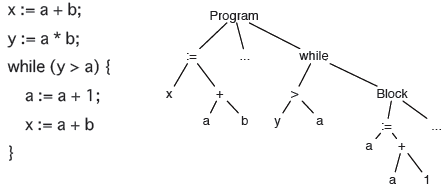
\includegraphics[width=0.8\textwidth]{ast.png}
	\caption{Пример программы и соответствующее ему АСД}%
\end{figure}

АСД строится по дереву разбора и отличается от него тем, что в нём отсутствуют узлы и рёбра для тех синтаксических правил, которые не влияют на семантику программы. Из-за этого в АСД отсутствует информация о форматировании кода, промежуточных узлах дерева и незначительных синтаксических элементах (скобки, точки с запятыми и т.д.). АСД обычно строится на поздних этапах работы компилятора, когда программа уже была обработана препроцессором и прошла проверку соответствия стандарту языка.

Для инструмента миграции программ больше подходит АСД. Информацию, которая была убрана во время составления АСД, можно восстановить, имея грамматику языка. Сложность, добавляемая в процесс превращение модели обратно в код, компенсируется упрощением анализатора и механизма трансформации.

Как правило, для построения АСД по исходному коду используют одну из существующих библиотек. Например, в случае языка Java есть выбор из следующих библиотек:

\begin{itemize}
\item Java Compiler Tree API - модуль, используемый стандартным компилятором Java для построения АСД. С одной стороны, <<официальный>> статус проекта гарантирует, что он будет корректно разбирать любой код на языке Java. С другой стороны, в нем отсутствуют некоторые важные возможности, например, модуль генерации кода.
\item Eclipse JDT - модуль, используемый средой разработки Eclipse. Имеет зависимости от самой среды разработки, поэтому его сложно использовать в отдельном (stand-alone) проекте.
\item ANTLR - генератор парсеров, использующий грамматики в форме Бэкуса-Наура. Не имеет модуля для генерации кода.
\item Javaparser. Позволяет генерировать код, поддерживает последнюю версию языка Java.
\end{itemize}

Кроме того, библиотека для построения АСД должна сохранять следующую информацию:
\begin{itemize}
\item Положении каждого терма в исходной программе (строка и столбец в файле)
\item Имя файла, из которого был взят терм
\end{itemize}

В результате проверки вышеперечисленных библиотек на соответствие требованиям был сделан вывод, что для задачи миграции программ лучше всего подходит библиотека Javaparser.

\section*{Выводы}
\addcontentsline{toc}{section}{Выводы}
В данной работе были рассмотрены подходы, которые могут использоваться для создания средства автоматизированной миграции программного кода на новый набор библиотек, а также инструменты, реализующие данные подходы. В результате был сделан вывод о том, что семантический подход является наиболее оптимальным для предложенной задачи.

Кроме того, были рассмотрены инструменты для смежной области трансформации программ. Были проанализированы модели кода, которые могут использоваться в средстве миграции. Наиболее подходящей моделью является АСД (абстрактное синтаксическое дерево).